\subsubsection{Trabajo de preparación}

\begin{figure}[ht]
    \centering
    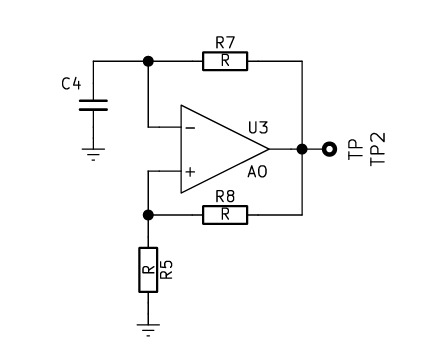
\includegraphics[width=0.5\textwidth]{multivibrador-astable.png}
    \caption{Multivibrador Astable con base en A.O}
    \label{fig:multivibrador-astable}
\end{figure}

\paragraph{Para el circuito de la figura \ref{fig:multivibrador-astable}, diseñar con el fin de obtener una oscilación de frecuencia 5.0kHz y amplitud 2V.\\}

Al usar un amplificador operacional UA741 alimentado con voltajes +VCC=10±1V y                     VEE= -10±1V este tendrá tensiones de saturación +Vsat = 8,005 V y –Vsat= -8,005 V, dichos valores fueron estudiados y comprobados en prácticas anteriores por lo cual serán utilizados como datos para esta práctica y para la práctica 3.3 del capítulo siguiente. 

\begin{equation}
    Vp = \frac{R_5}{R_5 + R_8} \cdot Vo_{\text{max}}
\end{equation}

Sustituyendo $Vp= 2V$ y $Vo = Vsat+ = 8V$ se tiene

$$
2 = \frac{R_5}{R_5 + R_8}8.1
$$

$$
2 R_5  + 2 R_8 = 8.1 R_5
$$

$$
2 R_8 = (8.1 - 2) R_5
$$


$$ R_8 = 3,05R_5$$

si $R_5 = 3.3k $

entonces 

$$ R_8 = 10k$$


La frecuencia requerida es de 5,0kHz, es decir:

\begin{equation}
    T = \frac{1}{f} = 0.2ms
\end{equation}

El periodo de un semi ciclo de la señal está dado por la carga exponencial del condensador (ecuación \ref{eq:tiempo_carga-exponencial}).

\[
t1 = - R_7 \mathcal{C}_4 \ln \left( \frac{V_{0} - V_{p_{max}}}{V_{o} - V_{p_{min}}} \right)
\]
\[
t1 = - R_7 \mathcal{C}_4 \ln \left( \frac{(1 - \frac{R_5}{R_5 + R_8})V_p}{(1 + \frac{R_5}{R_5 + R_8})V_p} \right)
\]

de donde tenemos: 

\[
t1 = - R_7 \mathcal{C}_4 \ln \left( \frac{R_8}{2 R_5 + R_8} \right)
\]

al ser el circuito simétrico, tenemos que 

\[
T = 2 t1 = - 2R_7 \mathcal{C}_4 \ln \left( \frac{R_8}{2 R_5 + R_8} \right)
\]



Asumiendo que $C_4 = 10nF$ se tiene

\[
R_7 = - \frac{T}{2C_4 \ln \left( \frac{R_B}{2R_S + R_g} \right)} = - \frac{0,2 \times 10^{-3}}{2 (100 \times 10^{-9}) \ln \left( \frac{1500}{2 \times 510 + 1500} \right)}
\]

$$R_7 = 22k\Omega$$


\begin{figure}[ht]
    \centering
    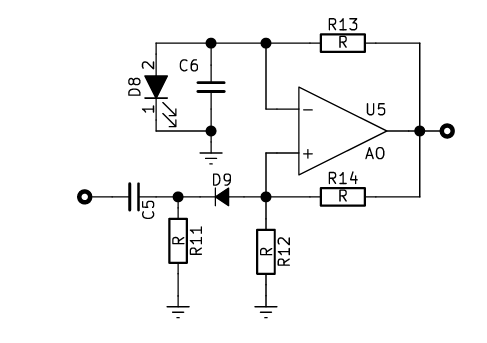
\includegraphics[width=0.5\textwidth]{multivibrador-monostable.png}
    \caption{Multivibrador Monostable con base en A.O}
    \label{fig:multivibrador-monostable}
\end{figure}


\paragraph{Para el circuito de la figura \ref{fig:multivibrador-monostable}, diseñar con el fin de obtener un tiempo de pulso de 10ms. }

El voltaje en la salida no inversora del amplificador (Vp), en el momento que ocurre el pulso negativo y D9 no conduce, está dado por la siguiente expresión: 

\[
V_{p3} = \frac{R_{12}}{R_{12} + R_{14}} Vo_{min}
\]

No hay condiciones de ganancia o de amplitud de las señales por lo que se tomarán valores arbitrarios para $R_{12}$ y $R_{14}$:

\begin{align}
    R_{12} = 5.1k \\
    R_14 = 10k
\end{align}

\[
V_{p3} = \frac{5.1k}{10k + 5.1k} (-8,005) = -6,38\,V
\]

$$V_p = 2.9$$

$R_{11}$ tiene que ser bastante mayor que $R_{12}$ para que el diodo se mantenga polarizado y también para que el paralelo $R_11 \parallel R_12$ no altere el comportamiento del circuito. Se tomará 

$$R_{11} = 100k$$

Para hallar el valor de $R_{13}$ se tiene vuelve a usar la ecuación \ref{eq:tiempo_carga-exponencial} de carga exponencial del condensador. Despejando $R_{13}$ se tiene:

\[
R_{13} = - \frac{t_c}{C_a \ln \left( \frac{V_{P3} - V_{SAT}}{V_{DB} - V_{SAT}} \right)} = - \frac{10 \cdot 10^{-3}}{(100 \cdot 10^{-9}) \ln \left( \frac{-6,38 - (-8,005)}{1,5 - (-8,005)} \right)} = 160k\Omega
\]

usando un valor comercial

$$R_{13} = 150k\Omega$$

\subsubsection{Simulaciones}

La ilustración \ref{fig:simulacion-multivibrador-astable-montaje} muestra la construcción del multivibrador astable en Multisim. En la ilustración \ref{fig:astable-forma-onda} se observa la forma de onda de la señal de salida $V_o$ y la señal en el condensador $V_p$ la cual tiene una forma parecida a una senoidal en vez de la forma exponencial de carga y descarga esperada.


\begin{ilustracion}[ht]
    \centering
    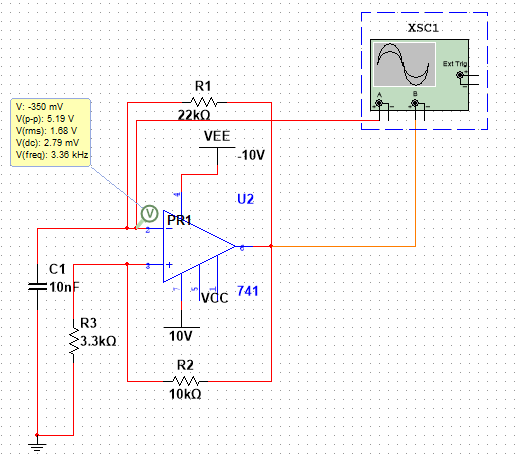
\includegraphics[width=0.7\textwidth]{simulaciones/montaje-astable.png}
    \caption{Simulación montaje del multivibrador astable en Multisim.}
    \label{fig:simulacion-multivibrador-astable-montaje}
\end{ilustracion}

\begin{ilustracion}[ht]
    \centering
    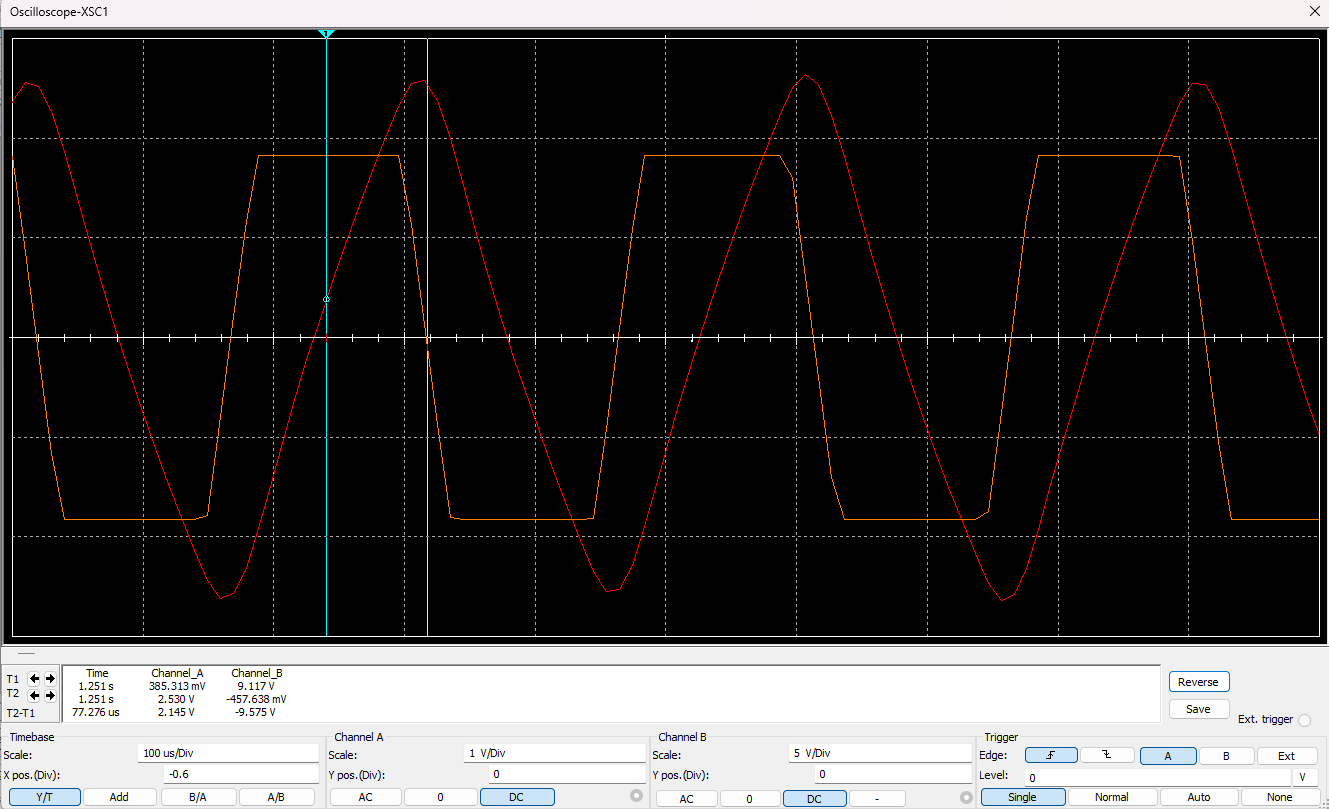
\includegraphics[width=0.8\textwidth]{simulaciones/forma-onda-astable.png}
    \caption{Simulación formas de onda ($V_o$, $V_p$) del multivibrador astable en Multisim.}
    \label{fig:astable-forma-onda}
\end{ilustracion}

La ilustración \ref{fig:simulacion-multivibrador-monostable-montaje} muestra la construcción del multivibrador monoestable en Multisim.

En la ilustración \ref{fig:monostable-forma-onda-freq-menor} se observa la forma de onda de la señal de salida $V_o$ la cual es cuadrada, la señal de pulso $V_g$ con un periodo mayor a 10ms y la señal de carga del condensador, la cual tiene la forma exponencial esperada. Se puede observar $V_c$ se mantiene en un estado estable ($V_o = V_{SAT+} =  8.005V$) hasta que ocurre un flanco ocasionado por el generador, el condensador se descarga y carga rápidamente a través de $R_{13}$ y $D_9$ en un tiempo de $11ms$ para luego volver a su zona estable.

En la ilustración \ref{fig:monostable-forma-onda-freq-mayor} se observa la forma de onda de la señal de salida $V_o$ y la señal de pulso $V_c$ en el condensador, esta vez se puede observar mientras el condensador está en su estado de carga y descarga a pesar de que ocurra otro pulso debido al generador, esto no altera el comportamiento de la carga, sino que espera a que el circuito vuelva a su estado estable para volver a descargarse cuando ocurra otro flanco.


\begin{ilustracion}[ht]
    \centering
    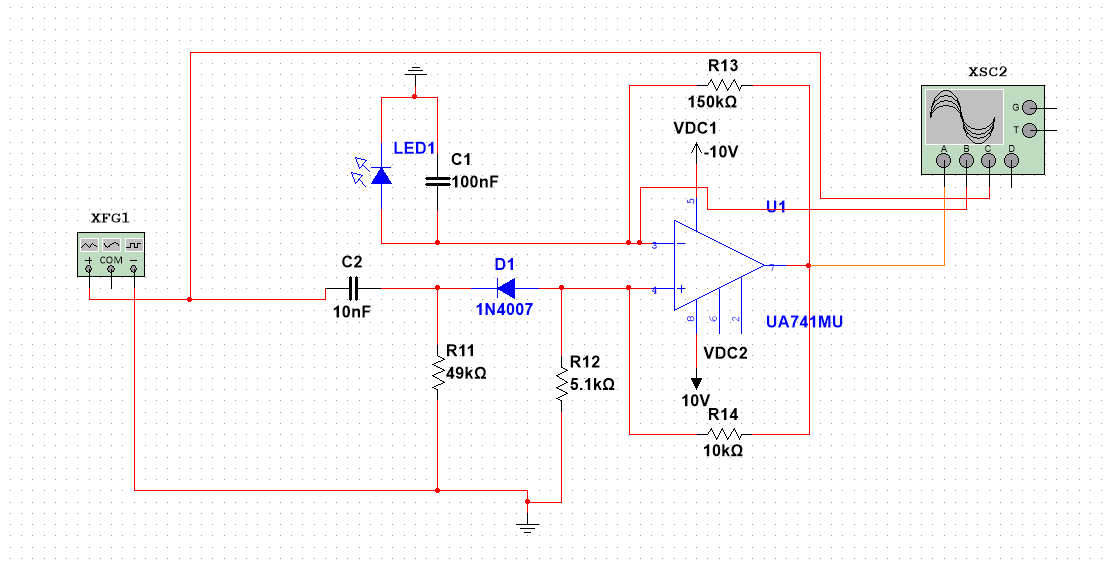
\includegraphics[width=0.7\textwidth]{simulaciones/montaje-monostable.png}
    \caption{Simulación montaje del multivibrador monoestable en Multisim.}
    \label{fig:simulacion-multivibrador-monostable-montaje}
\end{ilustracion}

\begin{ilustracion}[ht]
    \centering
    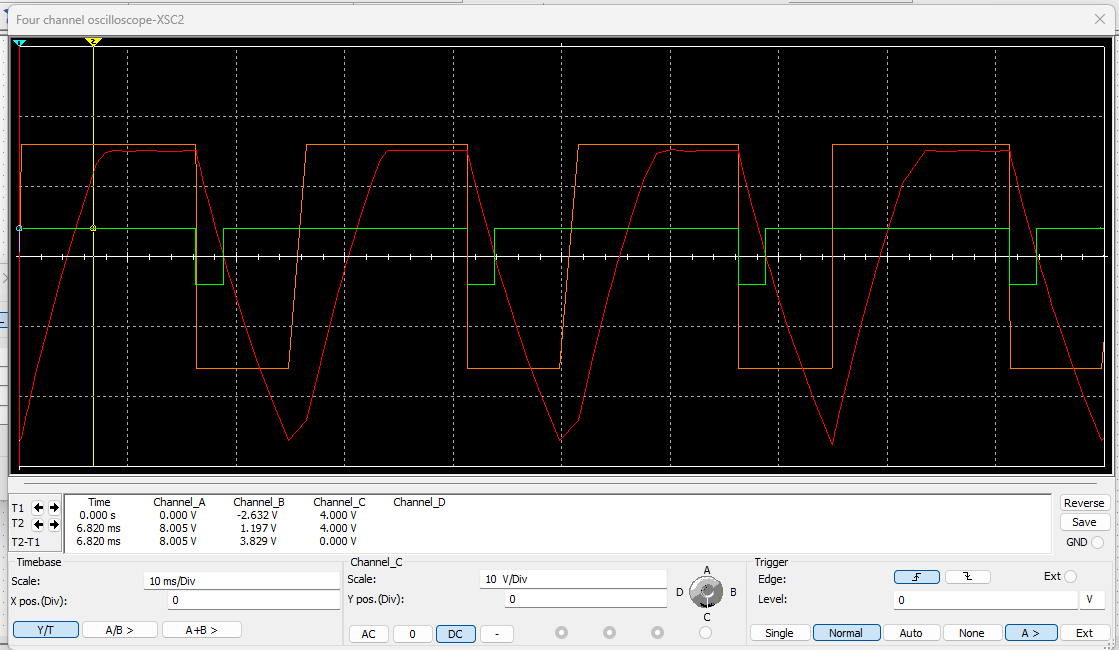
\includegraphics[width=0.8\textwidth]{simulaciones/forma-onda-monostable-freq-menor.png}
    \caption{Simulación formas de onda ($V_g$, $V_c$, $V_o$) del multivibrador monoestable cuando el periodo de la señal $V_g$ es menor a 10ms.}
    \label{fig:monostable-forma-onda-freq-menor}
\end{ilustracion}

\begin{ilustracion}[ht]
    \centering
    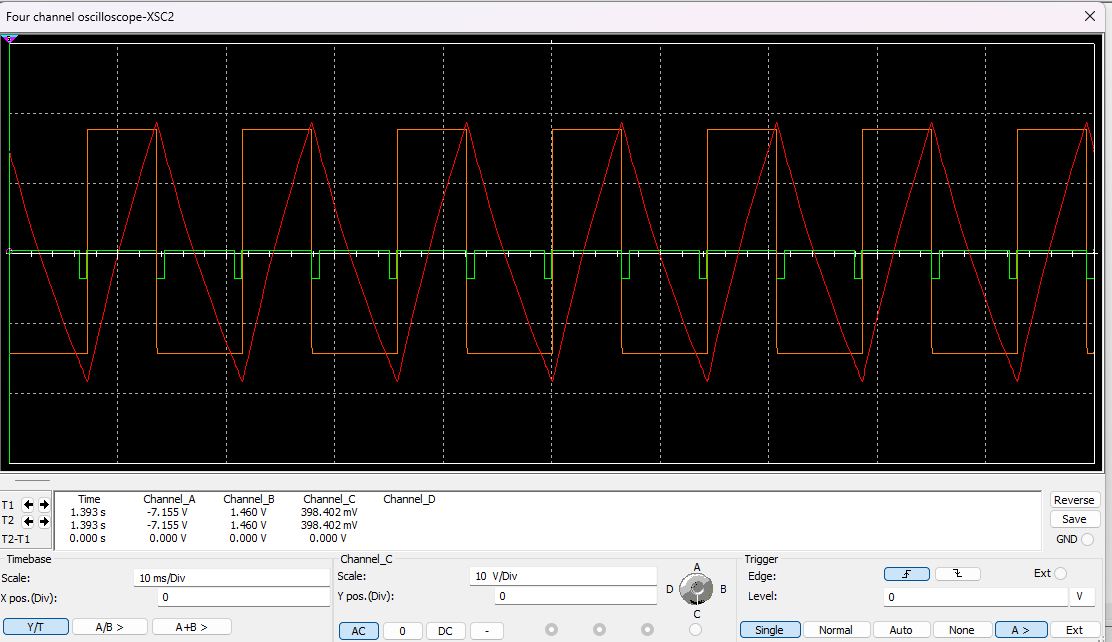
\includegraphics[width=0.8\textwidth]{simulaciones/forma-onda-monostable-freq-mayor.png}
    \caption{Simulación formas de onda ($V_g$, $V_c$, $V_o$) del multivibrador monoestable cuando el periodo de la señal $V_g$ es mayor a 10ms.}
    \label{fig:monostable-forma-onda-freq-mayor}
\end{ilustracion}
